\documentclass[tikz,border=4pt]{standalone}
\usepackage{tikz}
\usetikzlibrary{positioning,arrows.meta,fit,backgrounds,calc}

\definecolor{ctrlFill}{HTML}{dae8fc}
\definecolor{ctrlStroke}{HTML}{6c8ebf}
\definecolor{memFill}{HTML}{ffe6cc}
\definecolor{memStroke}{HTML}{d79b00}
\definecolor{calcFill}{HTML}{cce5ff}
\definecolor{calcStroke}{HTML}{4a86e8}
\definecolor{dataFill}{HTML}{d5e8d4}
\definecolor{dataStroke}{HTML}{82b366}
\definecolor{newStroke}{HTML}{b85450}
\definecolor{zoneStroke}{HTML}{888888}

\begin{document}
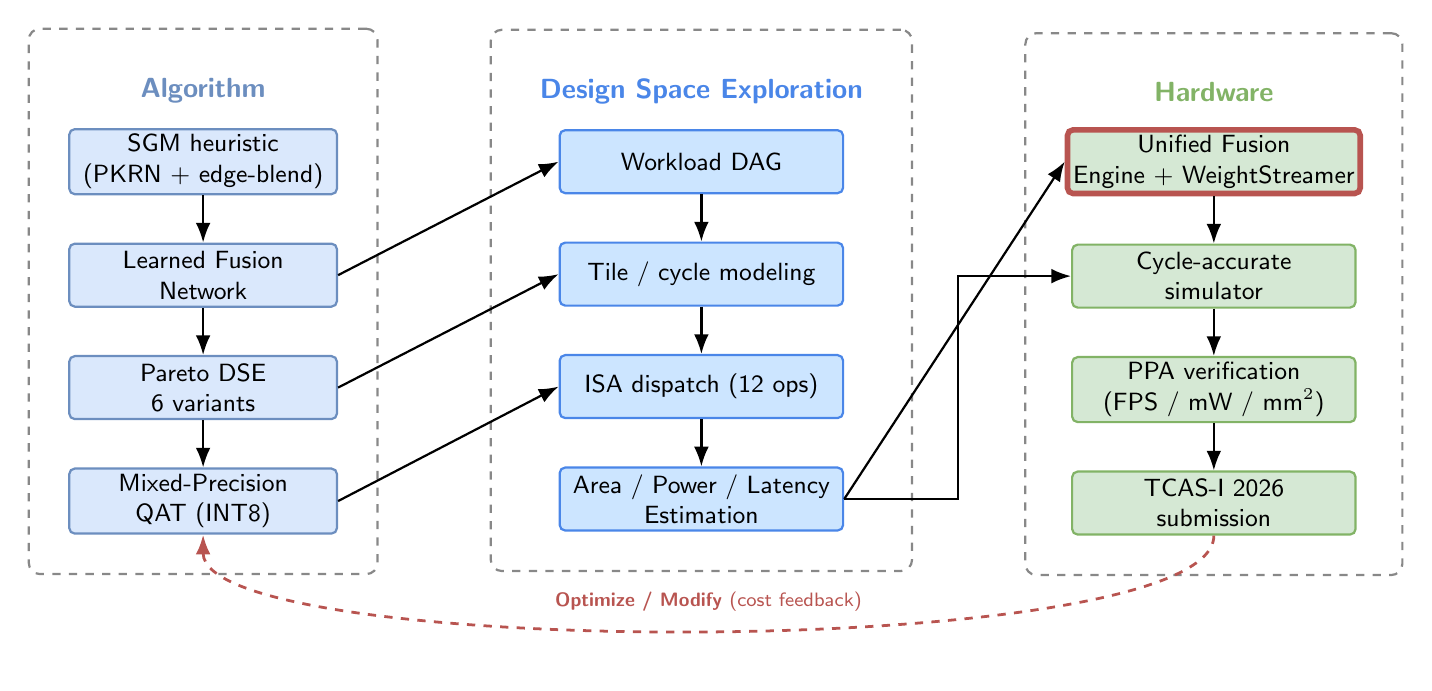
\begin{tikzpicture}[
  font=\small\sffamily,
  node distance=6mm,
  alg/.style   ={draw=ctrlStroke, fill=ctrlFill, rounded corners=2pt, thick, minimum width=34mm, minimum height=8mm, align=center, inner sep=2pt},
  dse/.style   ={draw=calcStroke, fill=calcFill, rounded corners=2pt, thick, minimum width=36mm, minimum height=8mm, align=center, inner sep=2pt},
  hw/.style    ={draw=dataStroke, fill=dataFill, rounded corners=2pt, thick, minimum width=36mm, minimum height=8mm, align=center, inner sep=2pt},
  hwnew/.style ={draw=newStroke,  fill=dataFill, rounded corners=2pt, line width=2pt, minimum width=36mm, minimum height=8mm, align=center, inner sep=2pt},
  zone/.style  ={draw=zoneStroke, dashed, rounded corners=4pt, thick, inner sep=5mm},
  arr/.style   ={-{Latex[length=2.5mm]}, thick},
  fbarr/.style ={-{Latex[length=2.5mm]}, thick, dashed, newStroke, line width=1pt},
]

% ============ Algorithm zone ============
\node[alg] (a1) at (0,0)        {SGM heuristic\\(PKRN + edge-blend)};
\node[alg, below=of a1] (a2)    {Learned Fusion\\Network};
\node[alg, below=of a2] (a3)    {Pareto DSE\\6 variants};
\node[alg, below=of a3] (a4)    {Mixed-Precision\\QAT (INT8)};

\node[above=2mm of a1, font=\normalsize\sffamily\bfseries, text=ctrlStroke] (atitle) {Algorithm};

% ============ DSE zone ============
\node[dse, right=28mm of a1] (d1) {Workload DAG};
\node[dse, below=of d1] (d2)     {Tile / cycle modeling};
\node[dse, below=of d2] (d3)     {ISA dispatch (12 ops)};
\node[dse, below=of d3] (d4)     {Area / Power / Latency\\Estimation};

\node[above=2mm of d1, font=\normalsize\sffamily\bfseries, text=calcStroke] (dtitle) {Design Space Exploration};

% ============ Hardware zone ============
\node[hwnew, right=28mm of d1] (h1) {Unified Fusion\\Engine + WeightStreamer};
\node[hw,    below=of h1] (h2)     {Cycle-accurate\\simulator};
\node[hw,    below=of h2] (h3)     {PPA verification\\(FPS / mW / mm$^2$)};
\node[hw,    below=of h3] (h4)     {TCAS-I 2026\\submission};

\node[above=2mm of h1, font=\normalsize\sffamily\bfseries, text=dataStroke] (htitle) {Hardware};

% ============ In-zone vertical arrows ============
\foreach \a/\b in {a1/a2, a2/a3, a3/a4, d1/d2, d2/d3, d3/d4, h1/h2, h2/h3, h3/h4} {
  \draw[arr] (\a) -- (\b);
}

% ============ Cross-zone arrows ============
\draw[arr] (a2.east) -- (d1.west);
\draw[arr] (a3.east) -- (d2.west);
\draw[arr] (a4.east) -- (d3.west);
\draw[arr] (d4.east) -- (h1.west);
\draw[arr] (d4.east) -| ($(d4.east)!0.5!(h2.west)$) |- (h2.west);

% ============ Dashed zones ============
\begin{scope}[on background layer]
  \node[zone, fit=(atitle) (a1) (a4), label={[anchor=south west, font=\scriptsize\sffamily, text=zoneStroke]above left:{}}] (zalg) {};
  \node[zone, fit=(dtitle) (d1) (d4)] (zdse) {};
  \node[zone, fit=(htitle) (h1) (h4)] (zhw)  {};
\end{scope}

% ============ Feedback loop: hw bottom -> alg top ============
\draw[fbarr] (h4.south) .. controls +(0,-16mm) and +(0,-16mm) .. node[midway, above=1mm, font=\scriptsize\sffamily, text=newStroke]{\textbf{Optimize / Modify} (cost feedback)} (a4.south);

\end{tikzpicture}
\end{document}
